\subsection{Monster and Boss}
The monsters in the game are unsynthesized entities which serve to make the game harder for the player. At their core they can attack the player and take damage. These two properties are shared with the boss, and is thus put in the \textit{IEnemy} interface. Both \textit{IMonster} and \textit{IBoss} implements the \textit{IEnemy} interface, and thus have the core functionality of an enemy. The monsters are interesting to us because they have to dispose their timers. If the timers are not disposed the monster will keep hitting the player after it has died although it would not seem to be in the room with the player. From the monster we can observe it is never the case that they become 'ghosts'. This can of course be explained with the fact that they are unsynthesized, so they always behave the same way. But we also note that the only time the monsters 'exit the game' is when they die, and this is also the time where they dispose their timers. The branch in the monsters \textit{Kill} method where they reach zero health is responsible for disposing the timers, and it is the only 'path' a monster can take to leave the game. The monster's \textit{Kill} method can be seen in \autoref{MonsterKill}. This is thus a very crucial part of the lifecycle for the monsters, one we do not want variations of. We thus observe that a safe way of ensuring a crucial part of the program is always there and always reachable is to make it unsynthesized.\\ \todo{Conclusion point}
The boss always spawn other actors, namely small monsters. This is done on a timer together with its other ability. It is thus also crucial for the boss to be able to dispose its timers. However, this time the entity we are working with \textit{is} synthesized, but the same concerns about always reaching specific parts of code is still present. To solve the timer disposing issue for the boss we used our observation about the monsters, and we decided that only one variation of the \textit{Kill} method should be created. This way we would always experience the same behaviour when the boss dies. The two \textit{Kill} methods are thus \textit{very} similar with small changes to what timers to dispose and what names to return from the call. Although, we do note that there is dead code in the boss' \textit{Kill} method due to the synthesis of one of two abilities. This is however a minor inconvenience as the field with the reference to the ability which is not synthesized is initialized to null, and the timer is only disposed if the field is not null.
\begin{figure}
	\centering
	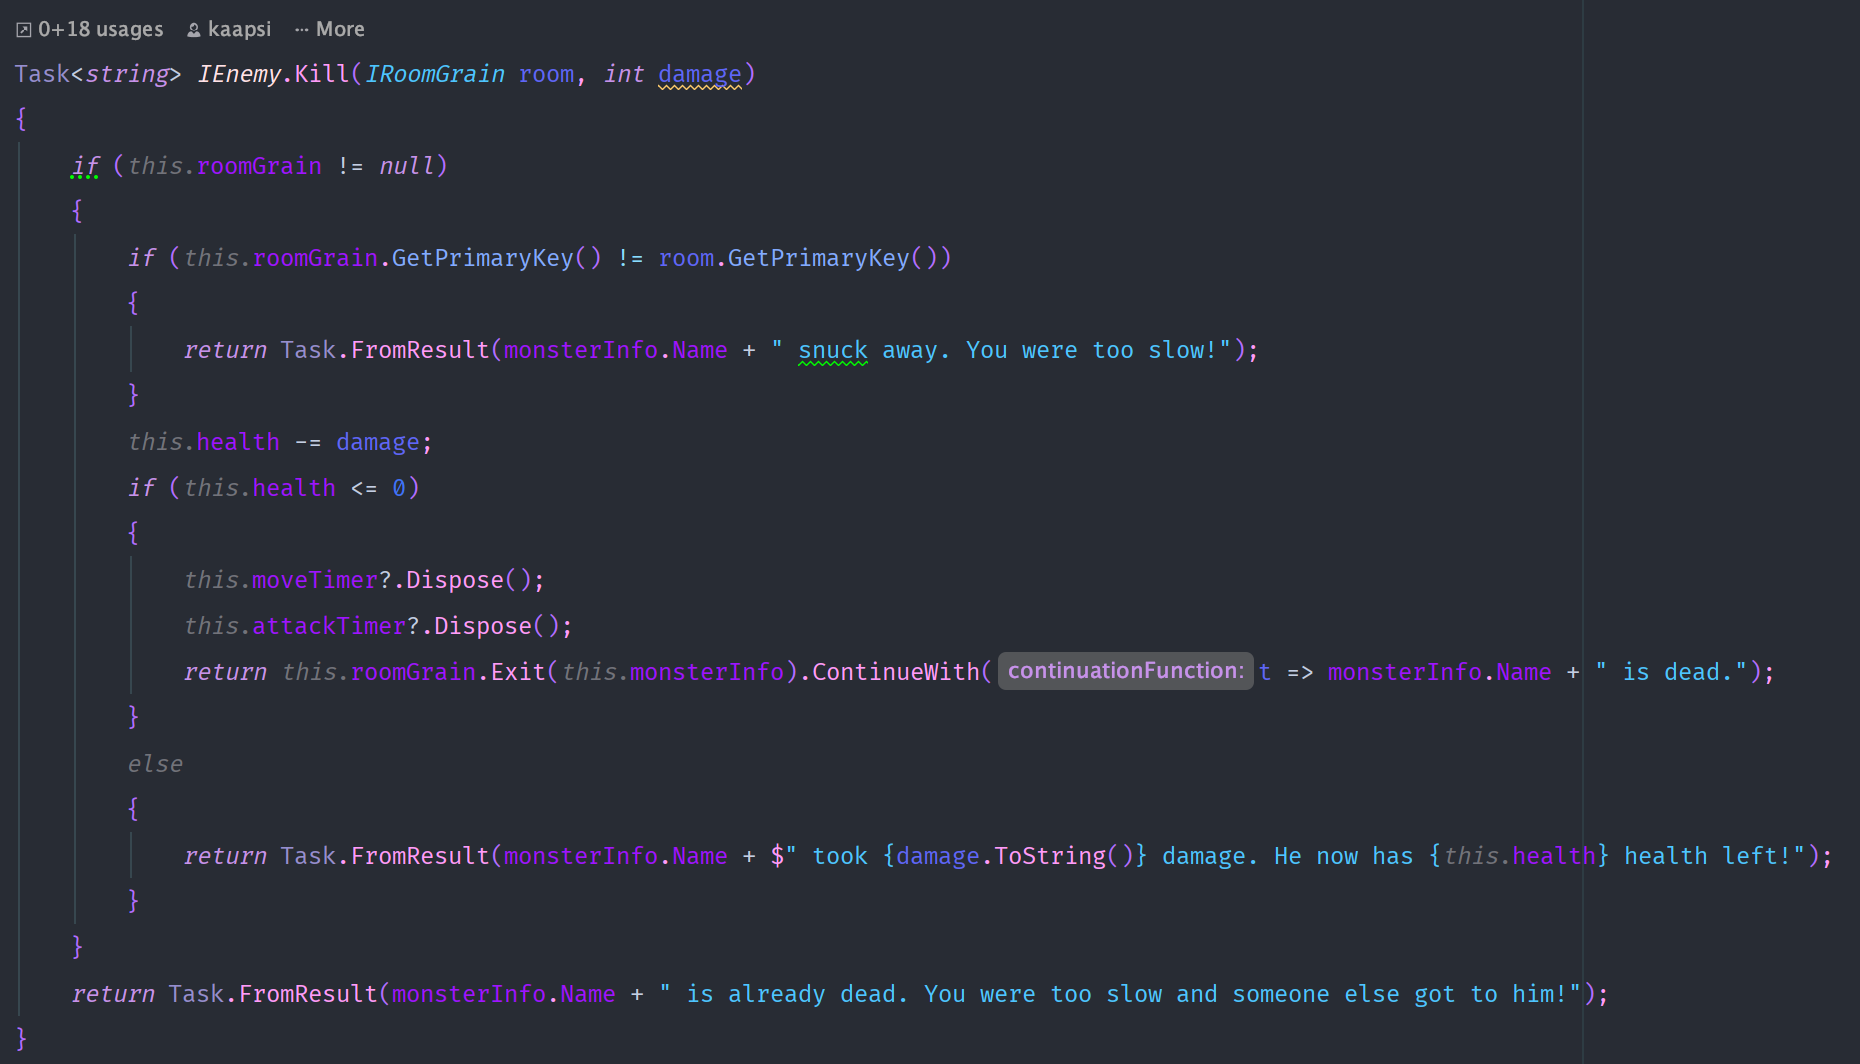
\includegraphics[width=\linewidth]{Materials/Decomposition/Boss/MonsterKill}
	\caption{The monster's method for taking damage.}
	\label{MonsterKill}
\end{figure}

\newpage

\begin{wrapfigure}{L}{0.55\linewidth}
	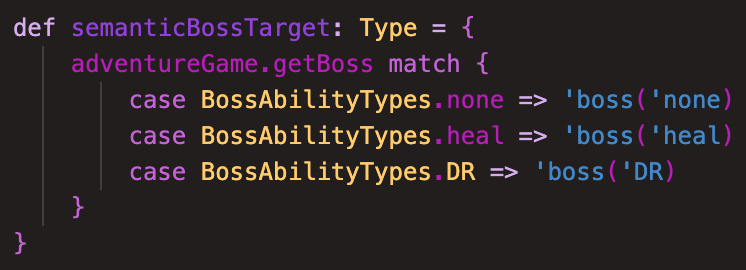
\includegraphics[width=\linewidth]{Materials/Decomposition/Boss/SemanticTarget}
	\caption{Depending on which ability is specified in the metalanguage, we will be looking for different intersections for the boss type.}
	\label{SemanticTargetExample}
\end{wrapfigure}
We found that the boss was a three-part entity, and is defined by its \textit{OnActivateAsync} method, its interaction with the room and perhaps most obviously its ability. We have named the semantic types for each part \textit{'bossOnActivateAsync'}, \textit{'bossRoomInteraction'} and \textit{'bossAbility'} respectively. All the semantic types are intersected by the kinding \textit{'bossAbility'} which can be either \textit{'heal'} or \textit{'DR'} (damage reduction). In our metalanguage we have defined a boss field which can take one of three enum values: \textit{'heal'}, \textit{'DR'} or \textit{'none'}. In \autoref{MetalanguageSetBoss} we see how we can set the boss to have the damage reduction ability in the metalanguage. In our semantic target we match our metalanguage defined boss field with the enum values and get the semantic type \textit{'boss'} intersected by the matching enum type back as seen in \autoref{SemanticTargetExample}.
\begin{figure}[H]
	\centering
	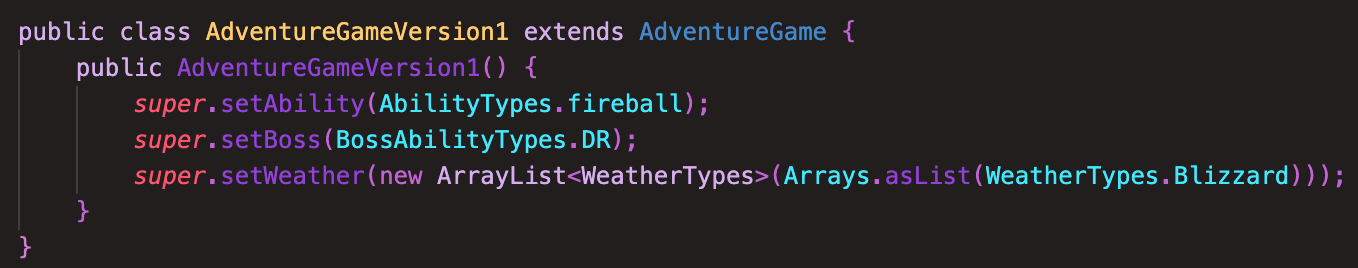
\includegraphics[width=0.95\textwidth]{Materials/Decomposition/Boss/MetalanguageSetBoss}
	\caption{Here we see how the boss is set to have the damage reduction ability in the metalanguage.}
	\label{MetalanguageSetBoss}
\end{figure}

For the semantic type \textit{'bossOnActivateAsync'} we have two combinators, one where the timer for the monster healing ability is started, and one where it is not. Otherwise there is a small additional setup for the boss which is the same for both combinators.\\
The two combinators for the abilities are also very simple. The variation with the heal ability implements the \textit{HealAdds} method whereas the variation with damage reduction is just an empty string. This is because there is no method for the damage reduction, its just a flag which is set whenever the boss spawns a new add.\\
This leaves us with the interaction between the room and the boss. To remove the damage reduction from the boss it needs to know when the adds die. For this we have added an observer like pattern between the room's \textit{Exit} method and the boss. Usually when implementing the observer pattern, several objects wants to know that something has changed to a single object, and so the single object broadcasts that this change has happened rather than the many objecting asking \textit{if} there have been a change. Here the room knows when the adds dies, namely when the \textit{Exit} method is called. We thus changed the \textit{Exit} method to call the boss' \textit{UpdateAdds} method. This is obviously dead code in the variations where we do not have any boss, and so we make a check for the boss being present in the room. The semantic type \textit{'bossRoomInteraction'} include the \textit{UpdateAdds} as it is here we set the damage reduction flag back to false, but it also includes the \textit{SpawnAdds} method as it is here we set the flag to true. Given \textit{SpawnAdds} calls the room's \textit{Enter} function (and thus has an interaction with the room) for the newly created monster we thought it would be fine to include both methods in the same combinator instead of creating more types and more complexity.\\
We here notice somewhat the same issue as with the player's abilities, namely that they do not share the same purpose. We see that the two abilities only changes a single line in \textit{SpawnAdds} and only a few lines in \textit{UpdateAdds} where the damage reduction flags are set. At first, one would think we could use dependency injection to define a common interface for boss abilities. But this would require the statement which sets the damage reduction flag in \textit{SpawnAdds} to be replaced by a call to an ability use, which would make the healing ability to heal each time an add is spawned which is not what we want. We here notice that the healing ability is on a timer whereas the damage reduction has a more event driven behaviour as it triggers when an add is spawned and when an add is killed, and the 'nature' of the two abilities are thus different. Using dependency injection would require one of the abilities to change 'nature' as either we would need to heal every time an add is spawned, or we would need to provide damage reduction on a timer. Changing the damage reduction to be on a timer which aligns with the timer for \textit{SpawnAdds} could work as it would remove the one-liner from \textit{SpawnAdds}, but we remove the synchronization of the damage reduction and the add spawning, and risk that an attack hits the boss between the add spawn and the damage reduction. We found that our implementation is the best solution to the issue although it to some extend limits the extendability of the boss.\\
For the variations with no boss we created a combinator which requires nothing, but creates a semantic type of \textit{'boss} intersected with \textit{'none} where the boss grain is simply empty.\\

One might now ask how we spawn the boss? This is done in \textit{'Adventure.cs'} where we add the method \textit{AddBoss}. This of course would also have to be synthesized and so if a boss is set in our metalanguage we have a combinator with our changes added, and if we are having a variation without a boss we have a combinator without our changes. We tried to merge this synthesis with the boss, but due to the limitation of only being able to create one file per job added to the CLS we had to split the synthesis in two.\\

In conclusion we found that the best way to ensure disposal of timers is to make it the only 'path' possible. We did this by only having one way for the monsters and the boss to exit the game, and that involved disposing their timers first. For safety we decided this was best done in unsynthesized code as this would ensure uniform behaviour no matter what variation we create.\\
We also see that spawning additional actors is no problem in a synthesized setting, and this can easily be achieved on a timer as with the boss. The only problem we encounter is created by us, and is how we have weaved the damage reduction ability into the add spawning. Although this approach to us seems better than the alternatives, it still limits the extendability of the boss.